\documentclass[]{article}
\usepackage[T1]{fontenc}
\usepackage{lmodern}
\usepackage{amssymb,amsmath}
\usepackage{fullpage}
\usepackage{ifxetex,ifluatex}
\usepackage{fixltx2e} % provides \textsubscript
% use microtype if available
\IfFileExists{microtype.sty}{\usepackage{microtype}}{}
\ifnum 0\ifxetex 1\fi\ifluatex 1\fi=0 % if pdftex
  \usepackage[utf8]{inputenc}
\else % if luatex or xelatex
  \usepackage{fontspec}
  \ifxetex
    \usepackage{xltxtra,xunicode}
  \fi
  \defaultfontfeatures{Mapping=tex-text,Scale=MatchLowercase}
  \newcommand{\euro}{€}
\fi
% Redefine labelwidth for lists; otherwise, the enumerate package will cause
% markers to extend beyond the left margin.
\makeatletter\AtBeginDocument{%
  \renewcommand{\@listi}
    {\setlength{\labelwidth}{4em}}
}\makeatother
\usepackage{enumerate}
\usepackage{graphicx}
% We will generate all images so they have a width \maxwidth. This means
% that they will get their normal width if they fit onto the page, but
% are scaled down if they would overflow the margins.
\makeatletter
\def\maxwidth{\ifdim\Gin@nat@width>\linewidth\linewidth
\else\Gin@nat@width\fi}
\makeatother
\let\Oldincludegraphics\includegraphics
\renewcommand{\includegraphics}[1]{\Oldincludegraphics[width=\maxwidth]{#1}}
\ifxetex
  \usepackage[setpagesize=false, % page size defined by xetex
              unicode=false, % unicode breaks when used with xetex
              xetex]{hyperref}
\else
  \usepackage[unicode=true]{hyperref}
\fi
\hypersetup{breaklinks=true,
            bookmarks=true,
            pdfauthor={Harshal Pandya and Brian Martin},
            pdftitle={CS677: Lab 1},
            colorlinks=true,
            urlcolor=blue,
            linkcolor=magenta,
            pdfborder={0 0 0}}
\setlength{\parindent}{0pt}
\setlength{\parskip}{6pt plus 2pt minus 1pt}
\setlength{\emergencystretch}{3em}  % prevent overfull lines
\setcounter{secnumdepth}{0}

\title{CS677: Lab 3}
\author{Brian Martin and Harshal Pandya}
\date{}

\begin{document}
\maketitle

Our system implements the provided spec: a pig2pig network in which pigs
collaborate to avoid impact with an adversarial bird. The pigs dynamically 
elect a leader amongst themselves and use Lamport's clocks for synchronization. 

\subsection{Actors}
We use the actor concurrency model to enable communication between machines. The
Actor model is a mathematical model of concurrent computation that
treats ``actors'' as the universal primitives of concurrent digital
computation: in response to a message that it receives, an actor can
make local decisions, create more actors, send more messages, and
determine how to respond to the next message received. Each actor is multi-threaded 
and can send/receive messages concurrently. Moreover, we can specify whether we want 
synchronous or asynchronous semantics.

\subsection{Leader Election}
We use the ring based leader election algorithm to enable the pigs to choose a leader dynamically.
Each pig gets a random 8-digit Id at start up and the pigs organize in a logical ring in an arbitrary order.
The network topology is completely connected which allows the pigs to reorganize into a new ring in the
event one of the nodes fails. Any pig can start the election. A message is circulated along the ring and every 
pig attaches its Id to the message and passes it on. When the initiator receives the message it, it picks the 
pig with the highest Id that is alive, informs everyone about the new leader. We use a timeout to figure whether 
a pig is down and move on if the pig does not respond within a particular interval.

\subsection{Clock Synchronization}
We use Lamport's clocks to order events across the pigs. When the leader initiates the game by sending the BirdApproaching 
message it sends along its current time to all pigs. The pigs use this value to update their clocks setting it to the max of remote 
and local clock. We simulate the network latency by incrementing the clock randomly (to a value up to 5) before processing the
bird approaching message. If the pig is able to move, the clock is advanced and the time is stored as Move Time. \\
After the time to target as specified by the bird has expired the leader sends a BirdLanded message to all pigs again with its time stamp. 
The pigs simulate the network delay and after comparing the time stamp, save it as Hit Time.\\
When the leader queries the pigs for their status, they respond by comparing these clock values to decide if they were able to move before the bird hit. 
Obviously, all this happens only if the pig is impacted by the bird's landing.  

\subsection{Game Map}

The game map is single-dimensional with pigs and columns placed
randomly. It is assumed that the bird is always launched from the left
(as in the original Angry Birds). The ratio of columns to pigs is at
most one.

\subsection{Assumed Physics}

We assume that certain behaviors for each element type:

\begin{itemize}
\item
  \textbf{Pig}: An impacted pig will fall to the right (as the bird
  always approaches from the left). If a pig falls onto another pig both
  are considered impacted, but the second pig does not change position
  on impact. If a pig is impacted while having a column to the right,
  then that column will also fall to the right, affecting any pig which
  may find itself in that position.
\item
  \textbf{Column}: If a column is impacted directly, then it falls to
  the right, only affecting any pig or column to its immediate right.
\end{itemize}

\subsection{Game Engine}

In our system the \emph{game engine} has several roles:

\begin{enumerate}[1.]
\item
  Map generation
\item
  Sending round-initiating trajectory message to the leader.
\item
  Querying the leader for the status of pigs. 
\end{enumerate}

\subsection{Pigs as Actors}

Each pig functions as an actor which can receive and act on several
message types, derived from the original specification. Some of them are listed below,
please refer to the doc provided for exhaustive list.

\begin{itemize}
\item
  \texttt{Trajectory(position: Int, birdLandingTime: Clock)} notifies the leader about the birds trajectory. That is, an estimate of the bird landing time as a (future) Lamport clock value.
\item
  \texttt{BirdApproaching(targetPosition: Int, timestamp: Clock)} This message provides is used by the leader to notify the other pigs of when the bird is expected to hit. Each pig attempts to move appropriately.
\item
  \texttt{Status()} Sent by the leader to query each pig about its safety after the bird landing. Each pig determines its own safety by comparing the Lamport clock value when that pig moved to the clock value for when the bird hit.
\item
  \texttt{Election()} Any pig can send this message to any other pig (including itself) to initiate a new election.
\end{itemize}

\subsection{Launching a bird}

A bird launch is described by the time the master picks a random target
and notifies the nearest pig about the trajectory. It then picks a
random time to target before sending an end game message thus signaling
that the bird has landed.

\section{Design Decisions / Trade-offs}

The pigs form a completely connected netowork topology and so hopcounts are not
required. However, this increases the complexity of the network and it may not
scale well for larger number of nodes.The pigs don't maintain any state apart
from their current locations in the world.

We choose ring based election algorithm since it involves no synchronization
issues and is fairly robust to failures. However we make a simplifying
assumption that a pig never goes down within a round. If this was not the case
we would need to back up the state of the leader and have it communicate to
each pig after every event so that it is up to date with the state of every
pig.

Lamport's clocks are convenient for this problem since they have much less
overhead than vector clocks. Since we are only comparing local timestamps and
the messages from the leader are broadcast, we can prove the correctness of the
partial ordering we care about.

We do not maintain a shared map data structure and hence the map is not updated
when the pigs move. This however saves the effort of maintaing a synchronous
thread-safe data structure that lives on the master and adds extra messages to
the system.

\section{Possible Improvements}

We could experiment with allowing the pigs to fail while a round is being played. 
In terms of the game logic, we could use a 2
dimensional world. Also we could make pigs move make space for pigs
being affected and have the effect of hits cascade beyond 2 positions.

\section{How to run the program}

We require \texttt{sbt}, the Scala Build Tool, to compile and run the code.

Our program can be run with:

\begin{enumerate}[1.]
\item
  \textbf{\texttt{./sbt11 numPigs worldSizeRatio}}: where numPigs is the number of pigs in the simulation and worldSizeRatio is the ratio of world:pigs. For example, to run with 10 pigs on a world of size 30 you would run: ./sbt11 10 3.
\end{enumerate}

\section{Experiments:}
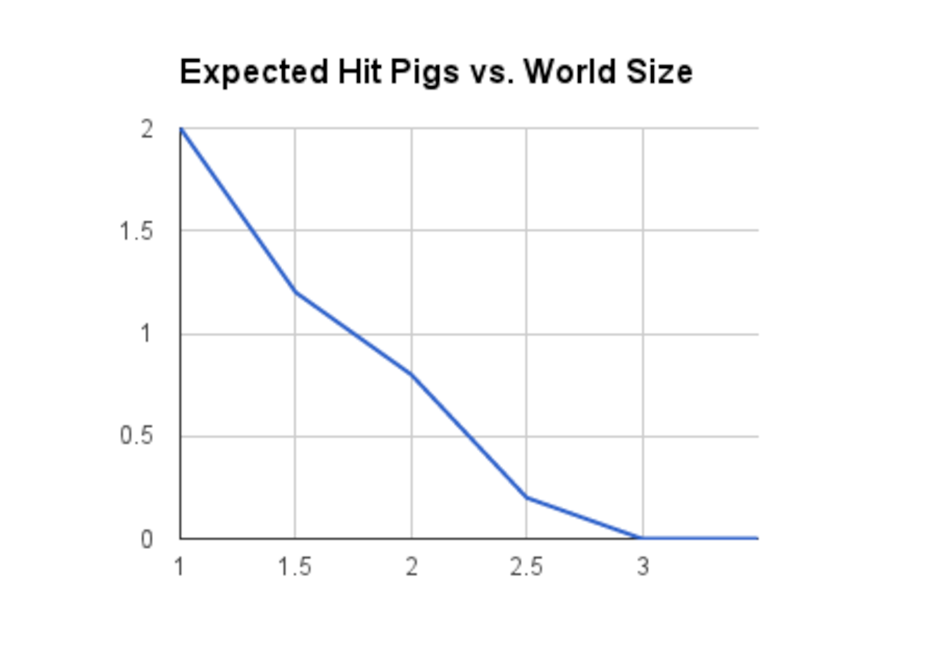
\includegraphics{figs/chart_1.pdf}
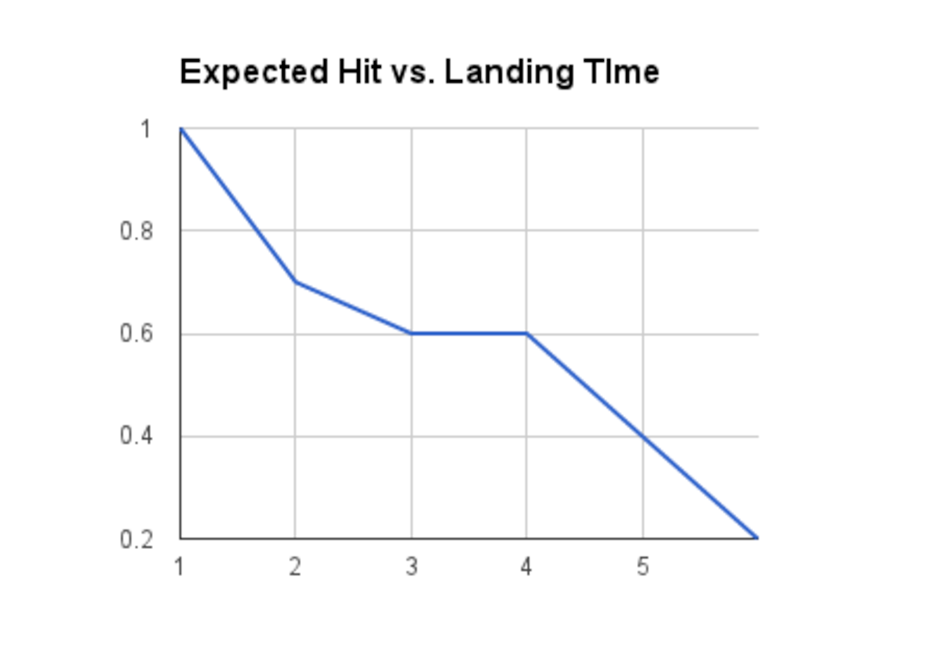
\includegraphics{figs/chart_2.pdf}

\pagebreak

\section{Test cases:}
We have a total of 6 test cases. 5 of these test whether the pigs respond to messages as expected. They are exemplified by the diagrams below. Note we produce a new leader at the start of each test case.\\
The Leader Election test case, tests the algorithm by first selecting the leader and then killing a leader and running the election again to produce a new leader. This is repeated twice and it can be seen that a new leader is picked successfully in the event of failure. 

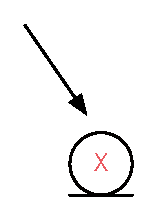
\includegraphics{figs/test1.pdf} 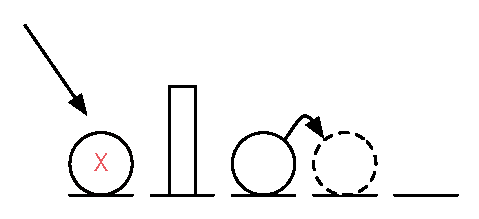
\includegraphics{figs/test2.pdf}
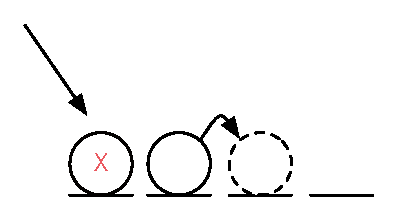
\includegraphics{figs/test3.pdf} 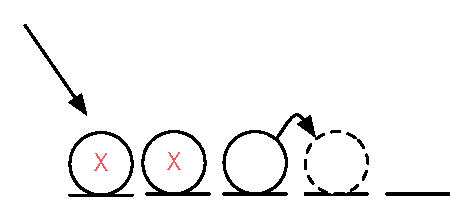
\includegraphics{figs/test4.pdf}
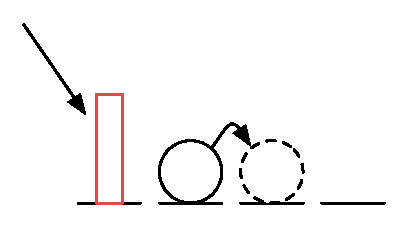
\includegraphics{figs/test5.pdf}


\section{Experiments}
We did 2 major experiments:
\begin{enumerate}[1.]
\item
  Expected number of pigs hit as function of the world size to number of pigs ratio.
\item
  Expected number of pigs hit as function of the the bird landing time.
\end{enumerate} 

\section{Sample Election Output:}

The following is the log of 10 pigs being started and an election occurring.
\tiny\begin{verbatim}
[info] INFO  [2013-04-13 02:50:16,723] com.github.harshal.distos.PigsRunner: Started pig on port: 10001
[info] INFO  [2013-04-13 02:50:16,725] com.github.harshal.distos.PigsRunner: Started pig on port: 10002
[info] INFO  [2013-04-13 02:50:16,725] com.github.harshal.distos.PigsRunner: Started pig on port: 10003
[info] INFO  [2013-04-13 02:50:16,725] com.github.harshal.distos.PigsRunner: Started pig on port: 10004
[info] INFO  [2013-04-13 02:50:16,725] com.github.harshal.distos.PigsRunner: Started pig on port: 10005
[info] INFO  [2013-04-13 02:50:16,725] com.github.harshal.distos.PigsRunner: Started pig on port: 10006
[info] INFO  [2013-04-13 02:50:16,725] com.github.harshal.distos.PigsRunner: Started pig on port: 10007
[info] INFO  [2013-04-13 02:50:16,725] com.github.harshal.distos.PigsRunner: Started pig on port: 10008
[info] INFO  [2013-04-13 02:50:16,726] com.github.harshal.distos.PigsRunner: Started pig on port: 10009
[info] INFO  [2013-04-13 02:50:16,726] com.github.harshal.distos.PigsRunner: Started pig on port: 10010
[info] DEBUG [2013-04-13 02:50:16,744] com.github.harshal.distos.Pig: 10001 recieved neighbor list: SetNeighbors(WrappedArray(10002, 10003, 10004, 10005, 10006, 10007, 10008, 10009, 10010))
[info] DEBUG [2013-04-13 02:50:16,803] com.github.harshal.distos.Pig: 10002 recieved neighbor list: SetNeighbors(WrappedArray(10003, 10004, 10005, 10006, 10007, 10008, 10009, 10010, 10001))
[info] DEBUG [2013-04-13 02:50:16,834] com.github.harshal.distos.Pig: 10003 recieved neighbor list: SetNeighbors(WrappedArray(10004, 10005, 10006, 10007, 10008, 10009, 10010, 10001, 10002))
[info] DEBUG [2013-04-13 02:50:16,866] com.github.harshal.distos.Pig: 10004 recieved neighbor list: SetNeighbors(WrappedArray(10005, 10006, 10007, 10008, 10009, 10010, 10001, 10002, 10003))
[info] DEBUG [2013-04-13 02:50:16,898] com.github.harshal.distos.Pig: 10005 recieved neighbor list: SetNeighbors(WrappedArray(10006, 10007, 10008, 10009, 10010, 10001, 10002, 10003, 10004))
[info] DEBUG [2013-04-13 02:50:16,927] com.github.harshal.distos.Pig: 10006 recieved neighbor list: SetNeighbors(WrappedArray(10007, 10008, 10009, 10010, 10001, 10002, 10003, 10004, 10005))
[info] DEBUG [2013-04-13 02:50:16,956] com.github.harshal.distos.Pig: 10007 recieved neighbor list: SetNeighbors(WrappedArray(10008, 10009, 10010, 10001, 10002, 10003, 10004, 10005, 10006))
[info] DEBUG [2013-04-13 02:50:16,988] com.github.harshal.distos.Pig: 10008 recieved neighbor list: SetNeighbors(WrappedArray(10009, 10010, 10001, 10002, 10003, 10004, 10005, 10006, 10007))
[info] DEBUG [2013-04-13 02:50:17,016] com.github.harshal.distos.Pig: 10009 recieved neighbor list: SetNeighbors(WrappedArray(10010, 10001, 10002, 10003, 10004, 10005, 10006, 10007, 10008))
[info] DEBUG [2013-04-13 02:50:17,045] com.github.harshal.distos.Pig: 10010 recieved neighbor list: SetNeighbors(WrappedArray(10001, 10002, 10003, 10004, 10005, 10006, 10007, 10008, 10009))
[info] DEBUG [2013-04-13 02:50:17,078] com.github.harshal.distos.PigsRunner: Sending DebugNeighbors..
[info] DEBUG [2013-04-13 02:50:17,079] com.github.harshal.distos.PigsRunner: Initiating an election..
[info] INFO  [2013-04-13 02:50:17,081] com.github.harshal.distos.Pig: 10001 Neighbors: 6aa0b301,e86b6882,304d79d2,0d6111de,1a57e8be,2108d235,c3923891,70de70bf,3a1c105f
[info] INFO  [2013-04-13 02:50:17,081] com.github.harshal.distos.Pig: 10007 Neighbors: c3923891,70de70bf,3a1c105f,32bc8116,6aa0b301,e86b6882,304d79d2,0d6111de,1a57e8be
[info] INFO  [2013-04-13 02:50:17,081] com.github.harshal.distos.Pig: 10005 Neighbors: 1a57e8be,2108d235,c3923891,70de70bf,3a1c105f,32bc8116,6aa0b301,e86b6882,304d79d2
[info] INFO  [2013-04-13 02:50:17,081] com.github.harshal.distos.Pig: 10008 Neighbors: 70de70bf,3a1c105f,32bc8116,6aa0b301,e86b6882,304d79d2,0d6111de,1a57e8be,2108d235
[info] INFO  [2013-04-13 02:50:17,081] com.github.harshal.distos.Pig: 10002 Neighbors: e86b6882,304d79d2,0d6111de,1a57e8be,2108d235,c3923891,70de70bf,3a1c105f,32bc8116
[info] INFO  [2013-04-13 02:50:17,081] com.github.harshal.distos.Pig: 10009 Neighbors: 3a1c105f,32bc8116,6aa0b301,e86b6882,304d79d2,0d6111de,1a57e8be,2108d235,c3923891
[info] INFO  [2013-04-13 02:50:17,081] com.github.harshal.distos.Pig: 10004 Neighbors: 0d6111de,1a57e8be,2108d235,c3923891,70de70bf,3a1c105f,32bc8116,6aa0b301,e86b6882
[info] INFO  [2013-04-13 02:50:17,081] com.github.harshal.distos.Pig: 10010 Neighbors: 32bc8116,6aa0b301,e86b6882,304d79d2,0d6111de,1a57e8be,2108d235,c3923891,70de70bf
[info] INFO  [2013-04-13 02:50:17,081] com.github.harshal.distos.Pig: 10006 Neighbors: 2108d235,c3923891,70de70bf,3a1c105f,32bc8116,6aa0b301,e86b6882,304d79d2,0d6111de
[info] INFO  [2013-04-13 02:50:17,081] com.github.harshal.distos.Pig: 10003 Neighbors: 304d79d2,0d6111de,1a57e8be,2108d235,c3923891,70de70bf,3a1c105f,32bc8116,6aa0b301
[info] DEBUG [2013-04-13 02:50:17,095] com.github.harshal.distos.Pig: Election from e86b6882 -> 304d79d2, succeeded...
[info] DEBUG [2013-04-13 02:50:17,095] com.github.harshal.distos.Pig: Election from 32bc8116 -> 6aa0b301, succeeded...
[info] DEBUG [2013-04-13 02:50:17,095] com.github.harshal.distos.Pig: Election from 6aa0b301 -> e86b6882, succeeded...
[info] DEBUG [2013-04-13 02:50:17,097] com.github.harshal.distos.Pig: Election from 304d79d2 -> 0d6111de, succeeded...
[info] DEBUG [2013-04-13 02:50:17,098] com.github.harshal.distos.Pig: Election from 0d6111de -> 1a57e8be, succeeded...
[info] DEBUG [2013-04-13 02:50:17,100] com.github.harshal.distos.Pig: Election from 1a57e8be -> 2108d235, succeeded...
[info] DEBUG [2013-04-13 02:50:17,102] com.github.harshal.distos.Pig: Election from 2108d235 -> c3923891, succeeded...
[info] DEBUG [2013-04-13 02:50:17,104] com.github.harshal.distos.Pig: Election from c3923891 -> 70de70bf, succeeded...
[info] DEBUG [2013-04-13 02:50:17,106] com.github.harshal.distos.Pig: Election from 70de70bf -> 3a1c105f, succeeded...
[info] INFO  [2013-04-13 02:50:17,107] com.github.harshal.distos.Pig: Election 1d33c08b finished: e86b6882 is the leader.
[info] DEBUG [2013-04-13 02:50:17,108] com.github.harshal.distos.Pig: Election from 3a1c105f -> 32bc8116, succeeded...
[info] DEBUG [2013-04-13 02:50:17,110] com.github.harshal.distos.Pig: 6aa0b301 setting leader to e86b6882
[info] DEBUG [2013-04-13 02:50:17,113] com.github.harshal.distos.Pig: e86b6882 setting leader to e86b6882
[info] DEBUG [2013-04-13 02:50:17,117] com.github.harshal.distos.Pig: 304d79d2 setting leader to e86b6882
[info] DEBUG [2013-04-13 02:50:17,120] com.github.harshal.distos.Pig: 0d6111de setting leader to e86b6882
[info] DEBUG [2013-04-13 02:50:17,123] com.github.harshal.distos.Pig: 1a57e8be setting leader to e86b6882
[info] DEBUG [2013-04-13 02:50:17,126] com.github.harshal.distos.Pig: 2108d235 setting leader to e86b6882
[info] DEBUG [2013-04-13 02:50:17,129] com.github.harshal.distos.Pig: c3923891 setting leader to e86b6882
[info] DEBUG [2013-04-13 02:50:17,132] com.github.harshal.distos.Pig: 70de70bf setting leader to e86b6882
[info] DEBUG [2013-04-13 02:50:17,135] com.github.harshal.distos.Pig: 3a1c105f setting leader to e86b6882
[info] DEBUG [2013-04-13 02:50:17,136] com.github.harshal.distos.Pig: 32bc8116 setting leader to e86b6882
\end{verbatim}
\normalsize

\end{document}
